% Attention weights over a short sentence: a softmax of SCORES per row.
\documentclass[tikz,border={72pt 6pt}]{standalone}  % side margins: a viewer that fits its width shows it whole
\usepackage[T1]{fontenc}
\usepackage{lmodern}
\definecolor{weight}{HTML}{2F5D9E}

\newif\ifcausal
\causalfalse  % true: a token attends only to itself and the tokens before it

\def\tokens{{"the","cat","sat","on","the","mat"}}
% scores[i][j]: how well query i matches key j
\def\scores{{{2.0,0.4,0.2,0.1,0.9,0.3},
             {0.6,2.2,0.9,0.2,0.3,0.8},
             {0.4,1.8,1.6,0.6,0.2,0.7},
             {0.2,0.5,1.4,1.5,0.4,0.9},
             {1.1,0.3,0.3,0.6,1.7,0.6},
             {0.3,1.0,0.8,1.2,0.9,2.1}}}

\begin{document}
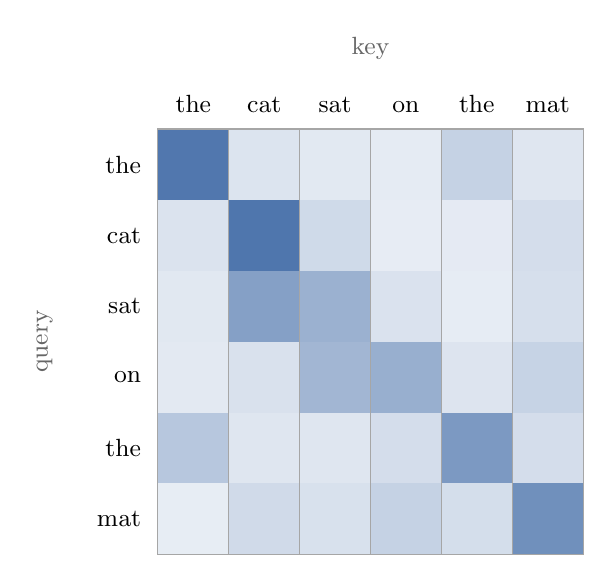
\begin{tikzpicture}[x=9mm, y=-9mm, font=\small]
  \foreach \i in {0,...,5} {
    % the row's softmax, over the keys it may see
    \pgfmathsetmacro{\total}{0}
    \foreach \j in {0,...,5} {
      \ifcausal\ifnum\j>\i\relax\else
        \pgfmathparse{\total + exp(\scores[\i][\j])}\xdef\total{\pgfmathresult}\fi
      \else
        \pgfmathparse{\total + exp(\scores[\i][\j])}\xdef\total{\pgfmathresult}\fi
    }
    \foreach \j in {0,...,5} {
      \ifcausal\ifnum\j>\i\relax
        \fill[black!7] (\j, \i) rectangle ++(1, 1);
      \else
        \pgfmathsetmacro{\w}{exp(\scores[\i][\j]) / \total}
        \pgfmathsetmacro{\shade}{min(100, 170 * \w)}
        \fill[weight!\shade!white] (\j, \i) rectangle ++(1, 1);
      \fi\else
        \pgfmathsetmacro{\w}{exp(\scores[\i][\j]) / \total}
        \pgfmathsetmacro{\shade}{min(100, 170 * \w)}
        \fill[weight!\shade!white] (\j, \i) rectangle ++(1, 1);
      \fi
    }
    \pgfmathsetmacro{\word}{\tokens[\i]}
    \node[anchor=east] at (-0.1, \i + 0.5) {\word};
    \node[anchor=south] at (\i + 0.5, -0.1) {\word};
  }
  \draw[black!35, step=1] (0, 0) grid (6, 6);
  \draw[black!35] (0, 0) rectangle (6, 6);
  \node[rotate=90, anchor=south, black!60] at (-1.35, 3) {query};
  \node[anchor=south, black!60] at (3, -0.85) {key};
\end{tikzpicture}
\end{document}
